% Copyright (C) 2013 - Michael Baudin
%
% This file must be used under the terms of the 
% Creative Commons Attribution-ShareAlike 3.0 Unported License :
% http://creativecommons.org/licenses/by-sa/3.0/

\chapter{Efficiency}

%%%%%%%%%%%%%%%%%%%%%%%%%%%%%%%%%%%%%%%%%%%%%%%%%%%%%%%%%%%%%%%%%%

\section{Error bounds}

	
	In this example, we show how the Quasi-Monte-Carlo (QMC) 
	integration outperforms the Monte-Carlo integration on a 
	typical example. 
	

	
	In general, the deterministic absolute error of QMC depends on 
$$
	\frac{(\log n)^s}{n}
$$
	where n is the number of points and s is the number 
	of dimensions.
	

	
	In general, the random absolute error of Monte-Carlo simulation 
	depends on 
$$
	\frac{1}{\sqrt{n}}
$$
	

	
	Hence, if s is moderate (i.e. from 1 to 20), the asymptotic 
	rate of convergence of QMC is much faster than the rate of Monte-Carlo. 
	

	
	Furthermore, it is known that, when the multi-dimensionnal function is purely additive, 
	i.e. when it is the sum of low-dimensionnal functions, 
	then QMC can reach its peak performance, which is very near 1/n 
	when s is moderate.
	
	
	
	The following script plots the Monte-Carlo and Quasi-Monte-Carlo convergence 
	rates, for increasing values of n and s=1,2 and 4. 
	
	
\lstset{language=scilabscript}
\begin{lstlisting}
scf();
n=2.^(1:30);
mcconv=1 ./sqrt(n);
qmcconv1=log(n).^1 ./n;
qmcconv2=log(n).^2 ./n;
qmcconv4=log(n).^4 ./n;
plot(n,mcconv,"k-");
plot(n,qmcconv1,"r-");
plot(n,qmcconv2,"g-");
plot(n,qmcconv4,"b-");
legend(["Monte-Carlo" ..
"Quasi-Monte-Carlo s=1" ..
"Quasi-Monte-Carlo s=2" ..
"Quasi-Monte-Carlo s=4" ..
]);
a=gca();
a.log_flags="lln";
xtitle("Convergence rate","Number of Simulations",..
"Absolute Error");
\end{lstlisting}

    
The previous script produces the figure \ref{fig-mcVsQmc-convergence}.

\begin{figure}[htbp]
\begin{center}
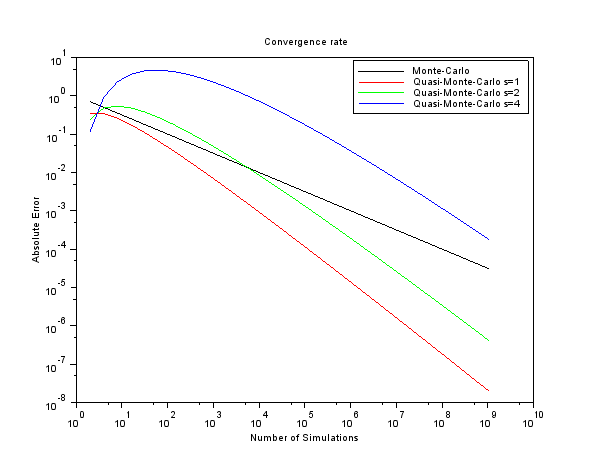
\includegraphics[width=15cm]{figures/mcVsQmc-convergence.png}
\end{center}
\caption{Theoretical convergence of Monte Carlo and Quasi-Monte Carlo.}
\label{fig-mcVsQmc-convergence}
\end{figure}
    
      We can see that the theoretical QMC convergence rate 
	  first increases, then decreases. 
	  It can be shown that the rate $\log(n)^s/n$ is increasing 
	  for n lower than exp(s), and then decreasing. 
	  For s=3, this is $n=\exp(3)$, which is almost equal to n=20, after 
	  which the asymptotic rate of QMC sets in. 
	  Hence, we see that the number of points n after which 
	  the asymptotic convergence sets in is larger when s increases. 
	  Moreover, we see that the accuracy of the integral as predicted 
	  by the QMC error bound is much larger when s increases. 
	  Fortunately, QMC can be, in some cases, 
	  much more accurate than the accuracy predicted by the error 
	  bound. 
    

%%%%%%%%%%%%%%%%%%%%%%%%%%%%%%%%%%%%%%%%%%%%%%%%%%%%%%%%%%%%%%%%%%

\section{The Ishigami example}
	
	We consider the Ishigami [1] example, which is often used as a 
	test case for sensitivity analysis. 
	This function depends on 3 
	input variables in the interval $[-\pi,\pi]$. 
	It is not purely additive, 
	but depends on interactions between $x_1$ and $x_3$. 
    Nevertheless, more that 75\% of the variance of f can be explained 
	by $x_1$ and $x_2$ alone, as can be explained by the first order 
	sensitivity indices computed after sensitivity analysis. 
	

\lstset{language=scilabscript}
\begin{lstlisting}
function y=ishigami(x)
  a = 7
  b = 0.1
  s1=sin(x(:,1))
  s2=sin(x(:,2))
  x34 = x(:,3).^4
  y(:,1) = s1 + a.*s2.^2 + b.*x34.*s1
endfunction
\end{lstlisting}

	
	In the following script, we use an increasing number of simulation 
	points and compare the absolute error between Monte-Carlo and QMC. 
	

\lstset{language=scilabscript}
\begin{lstlisting}
imax=18;
s=3;
integralExact=3.5;
// See the error with Monte-Carlo
errRand=[];
for i=1:imax
    npoints=2^i;
    x=distfun_unifrnd(-%pi,%pi,npoints,s);
    y=ishigami(x);
    integralApprox=mean(y);
    errRand(i)=abs(integralApprox-integralExact);
end
// See the error with Quasi Monte-Carlo
errQMC=[];
for i=1:imax
    npoints=2^i;
    u=lowdisc_ldgen(npoints,s);
    x=2*%pi*u-%pi;
    y=ishigami(x);
    integralApprox=mean(y);
    errQMC(i)=abs(integralApprox-integralExact);
end
scf();
n=2.^(1:imax);
mcconv=10 ./sqrt(n);
qmcconv=0.1*log(n).^s./n;
plot(n,errRand,"bo-");
plot(n,mcconv,"b-");
plot(n,errQMC,"ro-");
plot(n,qmcconv,"r-");
a=gca();
a.log_flags="lln";
legend(["Monte-Carlo" "MC Rate" ..
"Quasi-Monte-Carlo" "QMC rate"]);
xtitle("Quasi Monte-Carlo versus Monte-Carlo",..
"Number of simulations","Absolute Error");
\end{lstlisting}

    
  	  In the previous script, the constants 10 and 0.1 in 
	  \scivar{mcconv} and \scivar{qmcconv} are 
	  only there to be able to make the difference between the lines: 
	  only the slopes are meaningful in this convergence plot. 
The previous script produces the figure \ref{fig-qmc-ishigami}.

\begin{figure}[htbp]
\begin{center}
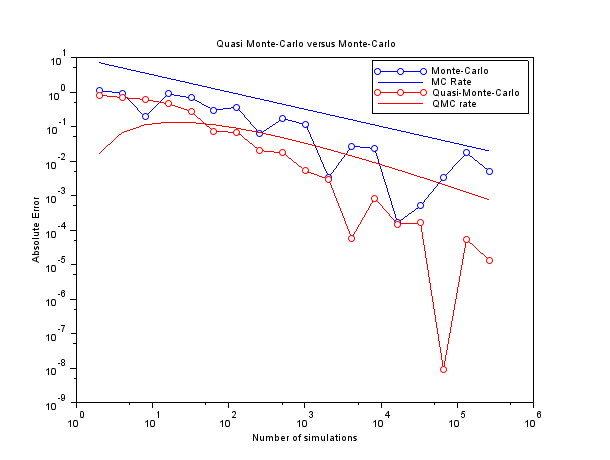
\includegraphics[width=15cm]{figures/qmc-ishigami.png}
\end{center}
\caption{Practical convergence of Monte Carlo and Quasi-Monte Carlo with the 
Ishigami test function.}
\label{fig-qmc-ishigami}
\end{figure}


      We can see that QMC outperforms MC in at least two senses. 
	  First, with 100 000 simulations, QMC can identify almost 5 
	  significant digits, while Monte-Carlo has only from 1 to 3 
	  significant digits. 
	  Second, the practical convergence rate of QMC is better 
	  than Monte-Carlo, and better than expected. 
	  We can see that it is almost equal to 1/n. 
	  This is a common situation, because the asymptotic 
	  bound given for low discrepancy sequences is just an 
	  upper bound. 
	  In general, the function is smoother than required by the 
	  low discrepancy sequence, and the achieved convergence is 
	  better than predicted by the theory. 
    

    
      The Ishigami is somewhere between difficult cases (where both QMC and MC 
	  fail) and easy cases (where QMC gives great results).
    
%%%%%%%%%%%%%%%%%%%%%%%%%%%%%%%%%%%%%%%%%%%%%%%%%%%%%%%%%%%%%%%%%%

\section{Efficiency of Quasi Monte-Carlo}
    
The actual efficiency of quasi-Monte-Carlo methods over crude Monte-Carlo
depends on the nature of the function to be integrated, 
the number of variables n and the number of dimensions s.



A typical failure of QMC involve functions which are highly 
oscillatory or discontinuous.



Another case of failure of QMC is for functions which are 
very different from an additive function. 
This happens when the function has high-order interations. 



QMC can perform differently depending on the structure of the 
interactions between input variables, especially when s is large.



In \cite{Sobol1994}, Sobol suggests
the following. If all the variables are
equally important and s is large (say, s>15), then there is no
advantage in switching to quasi-Monte-Carlo. However, if all the
variables are independent or if the dependence on xi decreases as
i increases (in other words, the initial coordinates are the leading ones),
one can expect a considerable benefit for QMC, even if s is
large (from s=10 to s=100, may be 1000).



Caflish, Morokoff and Owen defined the effective dimension of a function
in the superposition or in the truncation sense. Both these definitions
are making use of the functional ANOVA decomposition and lead
to global sensitivity indices, which normalized versions were first defined
by Sobol.
Functions with a small effective dimension d are easy to integrate as long
as the point set used has good properties for its projections over the first d
coordinates. The original Halton sequence should be quite sensitive to the
effective dimension d, since we know its projections deteriorate quickly as
the dimension increases.
    
